%% question-1.tex
%%

%% ==============================
\subsection{Diagramme de classe minimaliste du jeu}
\label{sec:question-1}
%% ==============================

Voici un diagramme de classe UML qui fixe les éléments principaux du jeu, c'est-à-dire le jeu en lui même, les joueurs, avatars, matchs, rencontres et les mondes.

Le jeu rassemble des joueurs, qui sauvegardent des avatars. Il possède des matchs qui sont constitués de rencontres qui on lieu dans des mondes. Les mondes sont possédés par le jeu.

\begin{figure}[h!]
	\centering
	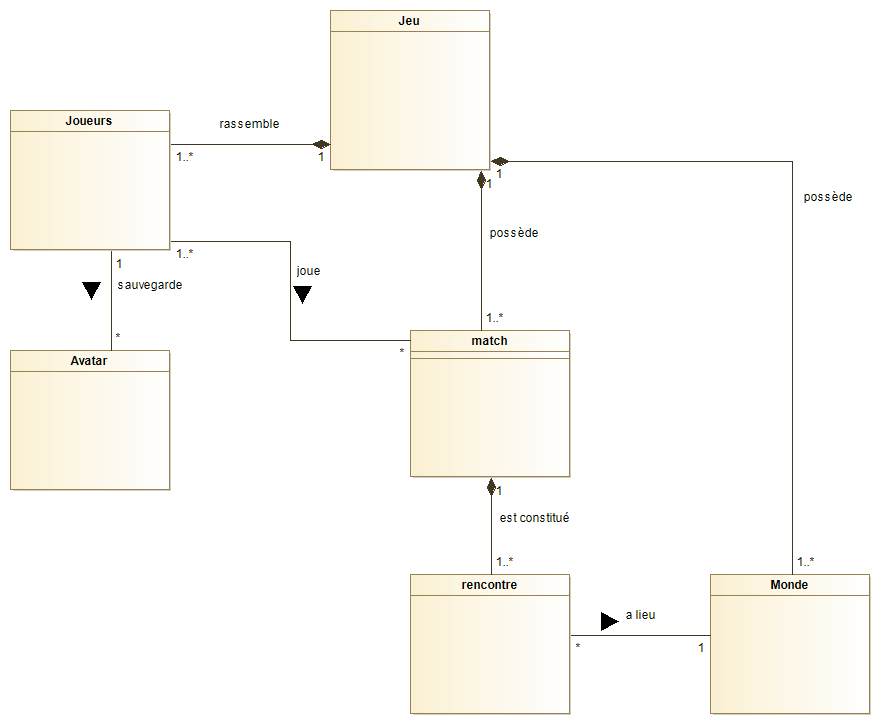
\includegraphics[width=250pt]{assets/diagrammeclassebase}
	\caption{Diagramme de classe des éléments principaux du jeu}
	\label{fig:diagrammeclassebase}
\end{figure}

\newpage